\chapter{Understanding User Engagement}

Next, we perform an engagement analysis of members on 7cot. Engagement analysis offers insights about the user and platform features that encourages members to return, listeners to stay active, and for members to have multiple, fruitful conversations. Such insights are practically important to help a platform retain new members and grow its community of listeners. They also identify qualities that encourage people to seek follow-up emotional support.

\section {Factors driving engagement}

We first relate the features and behaviors of members and its relationship to a measure of site engagement. Since sharing with listeners is the purpose of the service, we quantify engagement as the message rate of a member, that is, the average number of messages sent per day in conversations. We consider features and behaviors that, based on discussions with psychologists and designers at 7cot, may be related to engagement: (i) number of coins, growth points, and compassion hearts, which are gaming and progress measures related to a members reputation and experience; (ii) signup and last login date; (iii) reported distress level when they register; (iv) number of group chat messages; (v) number of page views from the 7cot Web and iOS applications; (vi) number of logins; (vii) number of conversation requests sent; (viii) number of self help page views; (ix) number of forum posts, views, and up-votes. Table ~\ref{table 5.1} gives the Pearson correlation coefficient between the features and a members’ message rates. The coefficients make clear that the gamification features of the platform (accumulated coins, hearts, and growth points) are strongly related to the engagement of a member. However, conversation messages sent by members directly increase growth points, giving this correlation little meaning. Member attributes and behaviors unrelated to communication (signup and last login date, distress level, page views, and help article views) exhibit virtually no correlation, suggesting that users dealing with any type and degree of emotional distress, at any time, exhibit similar levels of engagement on the site. 

\begin{table}
	\centering
	\begin{tabular}{c | c || c | c} 
		%\hline
		%Users & Count & Percentage \\ 
		%\hline\hline
	
		
	    Coins & 0.247 & Growth Points & 0.977 \\
	    Compassion Hearts & 0.243 & SignupDate & -0.009 \\
	    Last Login Date & 0.133 & Distress Level & 0.004 \\
	    Group Chat Msgs. & 0.120 & Page Views (Web) & -0.002 \\
	    Page Views (iOS) & -0.001 & Login Count & -0.001 \\
	    Conv. Requests & 0.001 & Self Help Views & 0.005 \\
	    Forum Posts & -0.001 & Forum Views & -0.001 \\
	    Forum Up Votes & 0.201 
		
	
	\end{tabular}
	\caption{Pearson correlation between message rate and user and behavior features}
	\label{table 5.1}
\end{table}

Many features exhibit little correlation with user engagement, but subsets of features may feature interactions that are. For example, users who exhibit a high distress level and submit many conversation requests may have a high level of engagement even though the features are individually not correlated. Instead of exhaustively exploring all multiway interactions, we consider a random forest model that predicts user engagement by a regression over all features. A random forest is an ensemble of decision trees, each of which is trained over different bootstraps of the data. During training, each tree is limited to the use of distinct small subsets of the features to make spitting decisions. The bootstraps, limited choice of features for tree splitting, and averaging of results across the tree ensemble ensures the forest does not overfit the data even for large N ~\cite{hastie2009unsupervised}. We compute the importance of each feature to the random forest regression model by the mean square error (MSE) of the random forest predictions against the actual engagement of every user. 

\newpage
We trained a random forest regression model using 75\% of the user data for a forest with N = 1000 trees and randomly choose 1/3 of the features for every tree splitting decision. The  figure ~\ref{fig:5.1}  shows the quantile plot and figure ~\ref{fig:5.2} shows the prediction scatter plots of the predicted and actual message rates for the 25\% of users not used to train the random forest. These figures demonstrate that the decision tree models engagement very well (R2 = 89\%), as the quantile plot shows a linear relationship between the distribution of the predicted and actual engagement rates up to the 60th quantile. The predicted vs. actual engagement rates in the Quantile plot   only show normally distributed errors for users with low engagement. 

\begin{figure}
	\centering %%%% this command is used to align center
	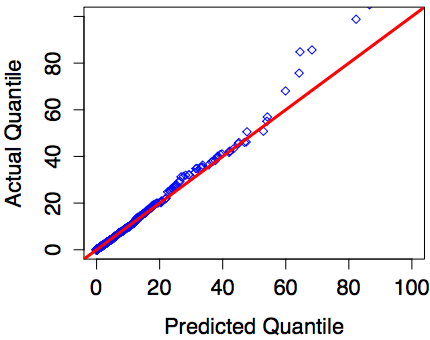
\includegraphics[width=4in]{Quantile.png} %include the saved image name in the braces as shown (VLSI_Chip.jpg)
	%%%% you can always adjust width of the image using command in square braces ([width=?in])
	\caption{Quantile Plot} 
	\label{fig:5.1}
\end{figure}

Since the random forest reasonably models the relationship between member and behavioral features, we use it for feature importance analysis. Figure ~\ref{fig:5.3} shows the percent increase in MSE of a random forest trained with data where each factor was individually perturbed across the training data. As anticipated by Table ~\ref{table 5.1}, the total number of growth points of a member is the most important factor for predicting user engagement due to its direct correspondence with her message rate. Members’ signup and last login dates are the next most important features, each of which increases MSE by over 20\% when they are perturbed. The signup date of a user is weakly anti-correlated with engagement according to Table ~\ref{table 5.1}, thus recent logins have a weak relationship to engagement. The number of messages sent in group chat is the next non-gaming related feature that is important for user engagement. This suggests that participating in group chats encourage users to become more engaged in their one-on-one conversations. It may be the case that users find group settings to be easier or less intimidating to participate in, and builds their confidence to have lengthy sessions with a listener. Finally, we note that the number of forum up votes introduces noise in the model, since perturbing this factor decreases the MSE of the random forest. One explanation may be that members who gain recognition for their forum posts may be disinclined to participate in conversations since they achieve recognition and perhaps satisfaction by only participating on the services forum. 

\begin{figure}
	\centering %%%% this command is used to align center
	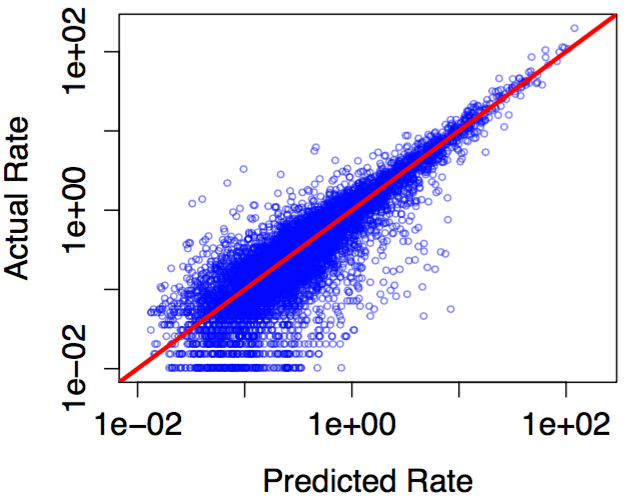
\includegraphics[width=4in]{Rate.png} %include the saved image name in the braces as shown (VLSI_Chip.jpg)
	%%%% you can always adjust width of the image using command in square braces ([width=?in])
	\caption{Predictions} 
	\label{fig:5.2}
\end{figure}


\begin{figure}
	\centering %%%% this command is used to align center
	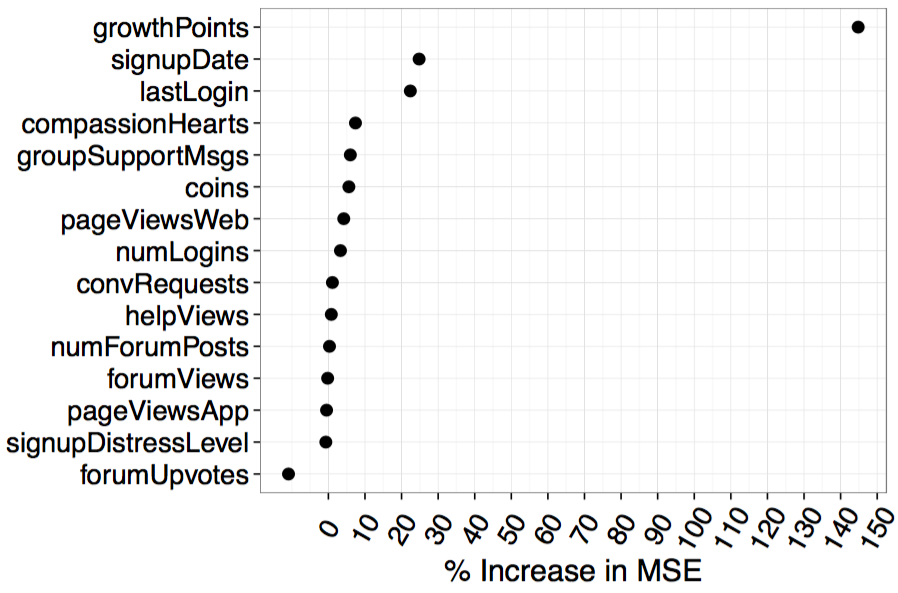
\includegraphics[width=4in]{FI.png} %include the saved image name in the braces as shown (VLSI_Chip.jpg)
	%%%% you can always adjust width of the image using command in square braces ([width=?in])
	\caption{Feature Importance in Random Forest Model} 
	\label{fig:5.3}
\end{figure}

\newpage
\section {New user engagement prediction}

New members to a service are often active for a brief period of time, then quickly become ‘inactive’ and never return or else they could become lurkers on the website who don't contribute any positively. Early identification of new users likely to become inactive or potential lurkers helps a platform identify those who could be encouraged to continue seeking help, or become listeners to bolster its community. Feature importance analysis of such a classifier performing such predictions may also reveal the user behaviors and attributes that promote people to return and seek follow-up emotional support.

We consider a random forest classifier that identifies if a member who, based on actions during her first two weeks on 7cot, will become an active user. Since there is lack of a standard definition for an ‘active’ user of a Web service, we consulted with 7cot administrators to define an active user as one who: (i) has been registered for at least six weeks; and (ii) has performed at least two actions on the service over the past month. We also define a ‘new user’ as one who has registered within the last two weeks. We identified all members who registered between May 7th (the first date user action data was recorded) and November 28th, 2014 (the end of our data set) and mark them as ‘active’ or ‘inactive’. We then collected the following actions they performed during their first two weeks on the site: (i) number of conversation requests and messages sent; (ii) number of forum posts made and viewed; (iii) number of logins performed; (iv) number of help page views; and (v) number of site pages accessed via 7cot’s Website and iOS app.

 21\% of the total members became active and 79\% became inactive or potential lurkers during this time period. We created a training set by randomly sampling 66\% of the registered members for a random forest classifier to predict if they are active. Trees are trained in a similar fashion to regression. Each tree yields its own prediction of if a member will be active or inactive given her actions during the first two weeks and a majority vote decides the class to be predicted. Due to the imbalance in the number of inactive and active members in the training data, we randomly oversample the minority class so that an equal number of inactive and active cases are provided for training, which is a common approach ~\cite{hastie2009unsupervised}. The trained random forest was tested over the 33\% of users not considered in the training set. The classifier achieves a very promising accuracy of 92.5\% and the ROC curve in Figure ~\ref{fig:5.4} demonstrates only a moderate false positive rate (ROC curves approaching the (0,1) corner of the plot are perfect classifiers; the y = x line represents a classifier that performs random guessing).

\begin{figure}
	\centering %%%% this command is used to align center
	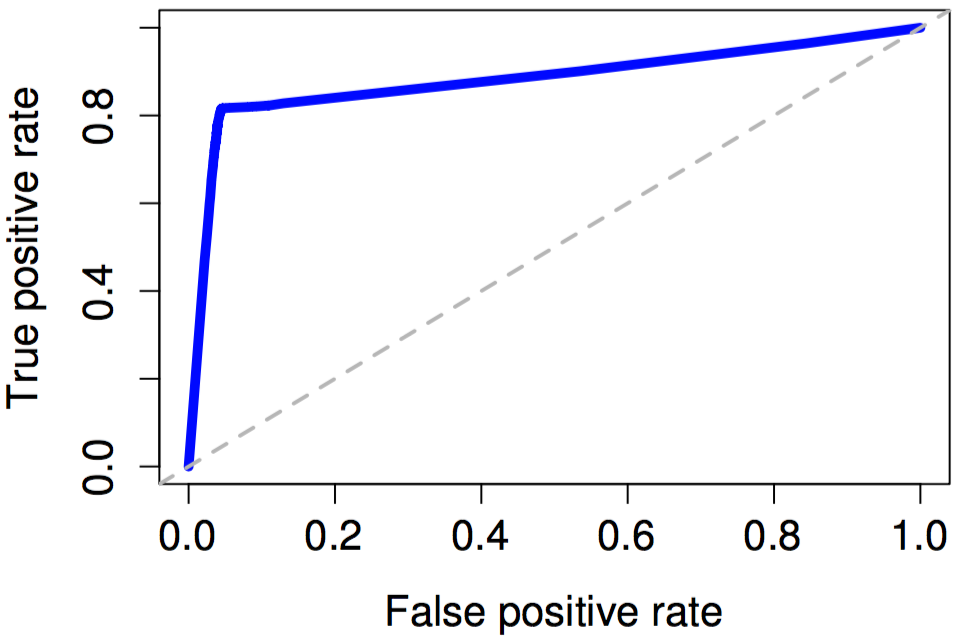
\includegraphics[width=4in]{ROC.png} %include the saved image name in the braces as shown (VLSI_Chip.jpg)
	%%%% you can always adjust width of the image using command in square braces ([width=?in])
	\caption{ROC Curve} 
	\label{fig:5.4}
\end{figure}

As before, we assess the importance of the factors used for predicting active users. Since the concept of MSE is incompatible with the notion of a binary classification decision, we instead consider the Gini index  of decision tree nodes in the forest ~\cite{hastie2009unsupervised}. The Gini index measures the average gain of purity by splits of a given variable. A Gini index close to zero suggests that the splitting rule at the parent divides the data into separate classes, which is a property of strong decision tree classifiers. We thus rank the importance of a factor by the average decrease of the Gini coefficient across all splits in all trees of the forest that involve it in figure ~\ref{fig:5.5}. It reveals that the number of messages sent in conversations and conversation requests submitted within the first two weeks are the actions that best predict whether a user will become active. We further examine the interaction between these two features by plotting the percentage of new users who became active and submitted  greater than x messages in their first two weeks in Figure . Each trend corresponds to subsets of members that also submitted less than the specified number of conversation requests. It shows how for small numbers of conversation requests, the total number of messages sent in one-on-one conversations strongly influences members to become active. But once approximately five conversations are created, the number of messages sent in a conversation loses its importance. This may be because new users that connect with greater numbers of listeners feel more obligated to return to these connections again in the future. On the other hand, when a user connects to only a few listeners, a stronger bond between them (i.e. more messages shared) is necessary to drive the member to return to the site.

\begin{figure}
	\centering %%%% this command is used to align center
	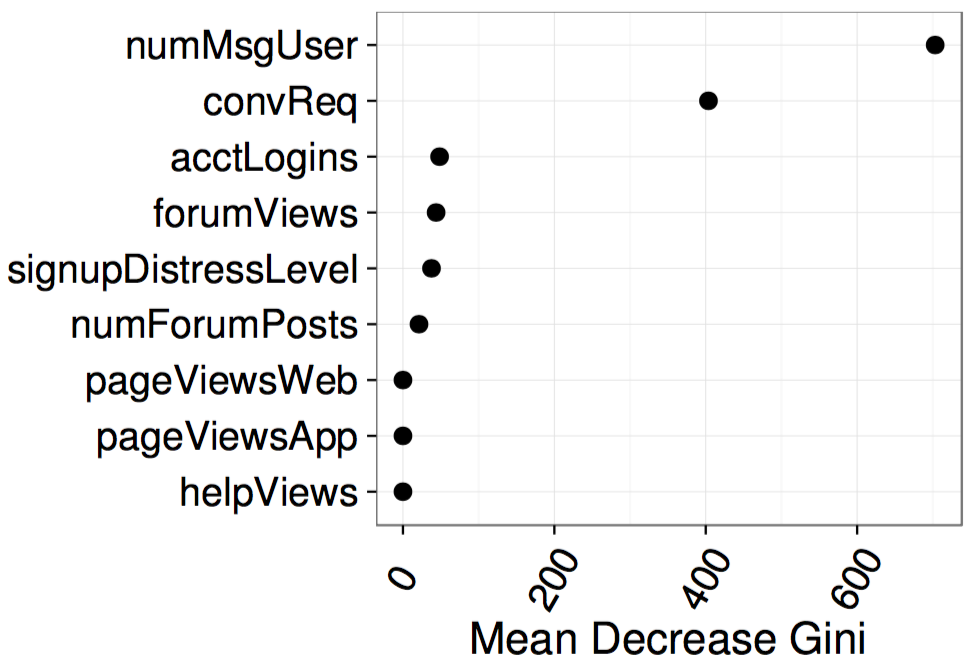
\includegraphics[width=4in]{Gini.png} %include the saved image name in the braces as shown (VLSI_Chip.jpg)
	%%%% you can always adjust width of the image using command in square braces ([width=?in])
	\caption{Gini Coefficient} 
	\label{fig:5.5}
\end{figure}

\newpage
Figure ~\ref{fig:5.6} also shows that the number of account logins performed, the user’s distress level, and activity related to the online forums within a member’s first two weeks are not major predictors of her becoming active. The frequency with which a member accesses the platform is thus unrelated to whether she will become an active member; what matters is not the number of times a member visits, but the quality or productivity of those visits as measured by the number of messages send and conversations requested. Furthermore, since members are equally likely to become active no matter their distress level, people suffering from both basic and complex problems may be equally willing to become active in online emotional support platforms. Finally, public spaces to post messages, such as forums, do not encourage new members to become active ones. This may be because forums serve as a less personal, more public medium of communication.

\begin{figure}
	\centering %%%% this command is used to align center
	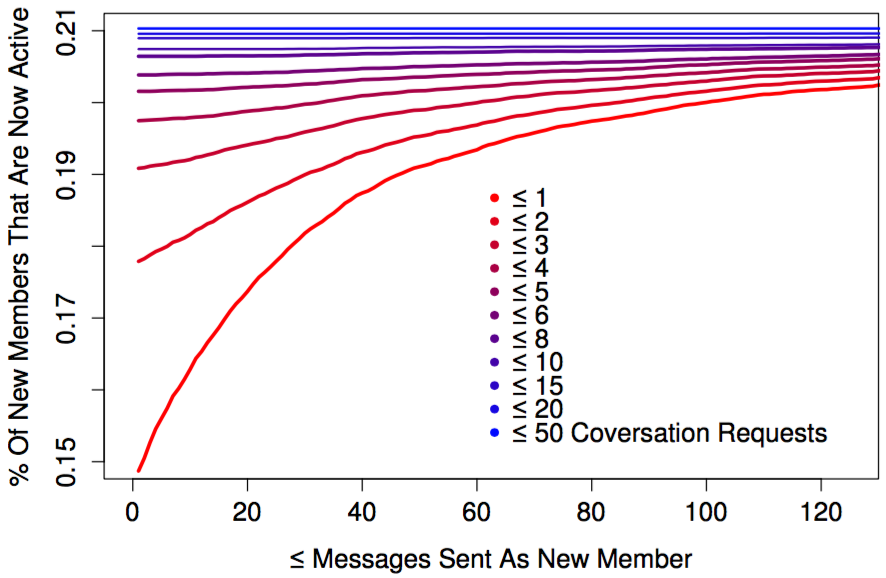
\includegraphics[width=4in]{Per.png} %include the saved image name in the braces as shown (VLSI_Chip.jpg)
	%%%% you can always adjust width of the image using command in square braces ([width=?in])
	\caption{Percent of Active Members retained} 
	\label{fig:5.6}
\end{figure}

\section{Summary of Findings}
In summary, this chapter identified a number of important insights about user engagement on this platform. Key takeaways from this study are :

\begin{itemize}
\item Users tend to exhibit similar level of engagement on the website irrespective of their emotional distress level or type.
\item The gamification mechanisms integrated in the platform (for eg. coins, growth points etc.) are very important for the user to stay engaged on the website. For instance, the listeners may find it very interesting to constantly try and level up their rank thereby gaining recognition and attention by the members on the website. This gives them additional motivation to get highly involved on the website apart from volunteering to help members facing distress.
\item Number of messages sent in conversations and conversation requests sent within the first two weeks best predict whether the user will become active in the long term.
\end{itemize} 